% ============================================================
% E3 FRAMEWORK ARCHITECTURE DIAGRAM
% ============================================================
% TikZ-based vector graphics for publication quality

\begin{figure*}[t]
\centering
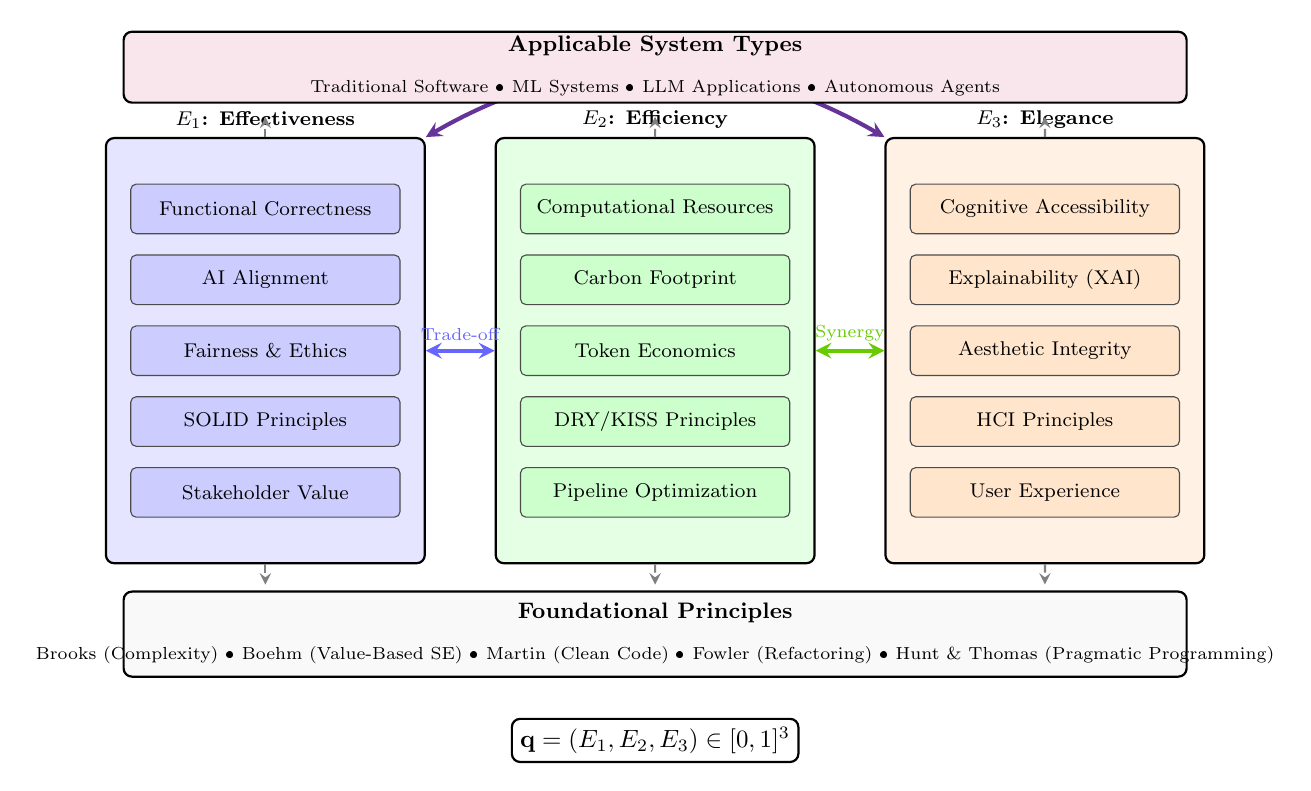
\begin{tikzpicture}[
    scale=0.9,
    transform shape,
    pillar/.style={
        rectangle,
        draw=black,
        thick,
        rounded corners=3pt,
        minimum width=4.5cm,
        minimum height=6cm,
        align=center,
        font=\small
    },
    component/.style={
        rectangle,
        draw=black!70,
        fill=white,
        rounded corners=2pt,
        minimum width=3.8cm,
        minimum height=0.7cm,
        align=center,
        font=\footnotesize
    },
    principle/.style={
        rectangle,
        draw=black!50,
        fill=gray!10,
        rounded corners=2pt,
        minimum width=3.5cm,
        minimum height=0.6cm,
        align=center,
        font=\scriptsize
    },
    arrow/.style={
        ->,
        thick,
        >=stealth
    },
    doublearrow/.style={
        <->,
        thick,
        >=stealth
    },
    label/.style={
        font=\footnotesize\bfseries
    }
]

% --- E1: Effectiveness Pillar ---
\node[pillar, fill=blue!10] (e1) at (0,0) {};
\node[label, above] at (e1.north) {$E_1$: Effectiveness};
\node[component, fill=blue!20] at (0,2) {Functional Correctness};
\node[component, fill=blue!20] at (0,1) {AI Alignment};
\node[component, fill=blue!20] at (0,0) {Fairness \& Ethics};
\node[component, fill=blue!20] at (0,-1) {SOLID Principles};
\node[component, fill=blue!20] at (0,-2) {Stakeholder Value};

% --- E2: Efficiency Pillar ---
\node[pillar, fill=green!10] (e2) at (5.5,0) {};
\node[label, above] at (e2.north) {$E_2$: Efficiency};
\node[component, fill=green!20] at (5.5,2) {Computational Resources};
\node[component, fill=green!20] at (5.5,1) {Carbon Footprint};
\node[component, fill=green!20] at (5.5,0) {Token Economics};
\node[component, fill=green!20] at (5.5,-1) {DRY/KISS Principles};
\node[component, fill=green!20] at (5.5,-2) {Pipeline Optimization};

% --- E3: Elegance Pillar ---
\node[pillar, fill=orange!10] (e3) at (11,0) {};
\node[label, above] at (e3.north) {$E_3$: Elegance};
\node[component, fill=orange!20] at (11,2) {Cognitive Accessibility};
\node[component, fill=orange!20] at (11,1) {Explainability (XAI)};
\node[component, fill=orange!20] at (11,0) {Aesthetic Integrity};
\node[component, fill=orange!20] at (11,-1) {HCI Principles};
\node[component, fill=orange!20] at (11,-2) {User Experience};

% --- Trade-off Arrows ---
\draw[doublearrow, blue!60, line width=1.5pt] (e1.east) -- (e2.west) 
    node[midway, above, font=\scriptsize] {Trade-off};
\draw[doublearrow, green!60!orange, line width=1.5pt] (e2.east) -- (e3.west) 
    node[midway, above, font=\scriptsize] {Synergy};
\draw[doublearrow, blue!60!orange, line width=1.5pt, bend left=30] (e1.north east) to 
    node[midway, above, font=\scriptsize] {Trade-off} (e3.north west);

% --- Foundation Layer ---
\node[rectangle, draw=black, thick, fill=gray!5, minimum width=15cm, minimum height=1.2cm, rounded corners=3pt] (foundation) at (5.5,-4) {};
\node[font=\small\bfseries] at (5.5,-3.7) {Foundational Principles};
\node[font=\scriptsize] at (5.5,-4.3) {Brooks (Complexity) • Boehm (Value-Based SE) • Martin (Clean Code) • Fowler (Refactoring) • Hunt \& Thomas (Pragmatic Programming)};

% --- System Types (Top) ---
\node[rectangle, draw=black, thick, fill=purple!10, minimum width=15cm, minimum height=1cm, rounded corners=3pt] (systems) at (5.5,4) {};
\node[font=\small\bfseries] at (5.5,4.3) {Applicable System Types};
\node[font=\scriptsize] at (5.5,3.7) {Traditional Software • ML Systems • LLM Applications • Autonomous Agents};

% --- Connecting lines to foundation and systems ---
\draw[arrow, gray, dashed] (e1.south) -- (0,-3.3);
\draw[arrow, gray, dashed] (e2.south) -- (5.5,-3.3);
\draw[arrow, gray, dashed] (e3.south) -- (11,-3.3);
\draw[arrow, gray, dashed] (e1.north) -- (0,3.3);
\draw[arrow, gray, dashed] (e2.north) -- (5.5,3.3);
\draw[arrow, gray, dashed] (e3.north) -- (11,3.3);

% --- Quality Vector Notation ---
\node[rectangle, draw=black, thick, fill=white, rounded corners=3pt, minimum width=4cm] at (5.5,-5.5) {
    $\mathbf{q} = (E_1, E_2, E_3) \in [0,1]^3$
};

\end{tikzpicture}
\caption{The E3 Framework Architecture. Three mutually reinforcing pillars—Effectiveness ($E_1$), Efficiency ($E_2$), and Elegance ($E_3$)—provide a comprehensive quality model applicable across deterministic and probabilistic software systems. Dashed arrows indicate grounding in foundational software engineering principles; bidirectional solid arrows indicate trade-off relationships between pillars.}
\label{fig:e3_framework}
\end{figure*}